\documentclass[tikz,border=2pt]{standalone}
\usepackage[scaled=0.92]{helvet}
\renewcommand\familydefault{\sfdefault}
\usepackage{sfmath}
\usepackage{amsmath}
\usetikzlibrary{arrows.meta,positioning,shapes.geometric,shapes.misc,fit,calc}

% PROTEUS documentation palette (docs/assets/proteus_architecture.svg)
\definecolor{pInk}{HTML}{10151B}
\definecolor{pLine}{HTML}{2A343D}
\definecolor{pFrame}{HTML}{5A6B7A}
\definecolor{pInterior}{HTML}{E23D28}
\definecolor{pStar}{HTML}{E0A32E}
\definecolor{pEscape}{HTML}{1B6FA8}
\definecolor{pOutgas}{HTML}{A03123}
\definecolor{pAtmos}{HTML}{4FA3D9}
\definecolor{pNo}{HTML}{C2362B}
\definecolor{pYes}{HTML}{2E8B57}
\definecolor{pIO}{HTML}{DDEBF5}

\begin{document}
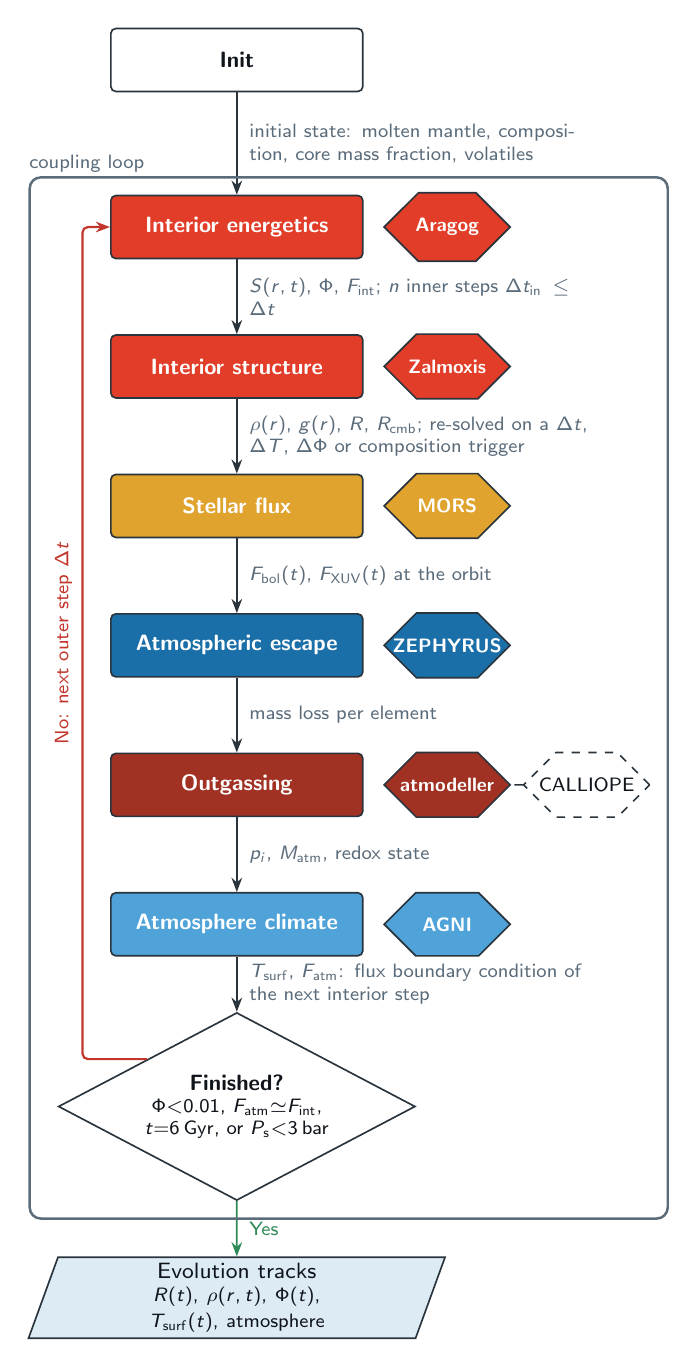
\begin{tikzpicture}[
  font=\footnotesize, text=pInk,
  node distance=9.5mm and 2.5mm,
  >={Stealth[length=1.8mm]},
  every path/.style={line width=0.6pt, draw=pLine},
  proc/.style={rectangle, rounded corners=1.8pt, draw=pLine, line width=0.6pt,
               minimum height=8mm, minimum width=32mm, text width=30mm,
               align=center, inner sep=2pt, text=white, font=\footnotesize\bfseries},
  mod/.style={chamfered rectangle, chamfered rectangle corners=all,
              chamfered rectangle xsep=2.2mm, chamfered rectangle ysep=3.25mm,
              draw=pLine, line width=0.6pt, minimum height=6.5mm, minimum width=16mm,
              inner sep=0pt, text=white, font=\scriptsize\bfseries},
  ref/.style={mod, dashed, fill=white, text=pInk, font=\scriptsize},
  dec/.style={diamond, aspect=1.9, draw=pLine, fill=white, inner sep=0.5pt,
              text width=29mm, align=center, font=\scriptsize},
  io/.style={trapezium, trapezium left angle=70, trapezium right angle=110, draw=pLine,
             fill=pIO, minimum height=7mm, text width=44mm, align=center, inner sep=2pt},
  lab/.style={font=\scriptsize, text=pFrame, inner sep=0pt, anchor=west,
              text width=44mm, align=left},
]

% spine
\node[proc, fill=white, text=pInk] (init) {Init};
\node[proc, fill=pInterior, below=13mm of init] (energ) {Interior energetics};
\node[proc, fill=pInterior, below=of energ] (struct) {Interior structure};
\node[proc, fill=pStar, below=of struct] (stellar) {Stellar flux};
\node[proc, fill=pEscape, below=of stellar] (escape) {Atmospheric escape};
\node[proc, fill=pOutgas, below=of escape] (outgas) {Outgassing};
\node[proc, fill=pAtmos, below=of outgas] (climate) {Atmosphere climate};
\node[dec, below=7mm of climate] (stop) {\textbf{\footnotesize Finished?}\\[0pt]
  $\Phi{<}0.01$, $F_\mathrm{atm}{\simeq}F_\mathrm{int}$,\\ $t{=}6\,\mathrm{Gyr}$, or $P_\mathrm{s}{<}3\,\mathrm{bar}$};
\node[io, below=7mm of stop] (out) {Evolution tracks\\[-1pt]
  {\scriptsize $R(t)$, $\rho(r,t)$, $\Phi(t)$, $T_\mathrm{surf}(t)$, atmosphere}};

% modules (flat hexagons, as in the documentation schematic)
\node[mod, fill=pInterior, right=of energ] (m1) {Aragog};
\node[mod, fill=pInterior, right=of struct] (m2) {Zalmoxis};
\node[mod, fill=pStar, right=of stellar] (m3) {MORS};
\node[mod, fill=pEscape, right=of escape] (m4) {ZEPHYRUS};
\node[mod, fill=pOutgas, right=of outgas] (m5) {atmodeller};
\node[ref, right=1.5mm of m5] (m5r) {CALLIOPE};
\node[mod, fill=pAtmos, right=of climate] (m6) {AGNI};
\draw[dashed] (m5r) -- (m5);

% spine arrows
\draw[->] (init) -- (energ);
\draw[->] (energ) -- (struct);
\draw[->] (struct) -- (stellar);
\draw[->] (stellar) -- (escape);
\draw[->] (escape) -- (outgas);
\draw[->] (outgas) -- (climate);
\draw[->] (climate) -- (stop);
\draw[->, draw=pYes] (stop) -- (out);

% edge labels: centred in each gap, right of the arrow, so they clear every box
\node[lab] at ($(init.south)!0.5!(energ.north)+(1.5mm,0)$)
  {initial state: molten mantle, composition, core mass fraction, volatiles};
\node[lab] at ($(energ.south)!0.5!(struct.north)+(1.5mm,0)$)
  {$S(r,t)$, $\Phi$, $F_\mathrm{int}$; $n$ inner steps $\Delta t_\mathrm{in}\le\Delta t$};
\node[lab] at ($(struct.south)!0.5!(stellar.north)+(1.5mm,0)$)
  {$\rho(r)$, $g(r)$, $R$, $R_\mathrm{cmb}$; re-solved on a $\Delta t$, $\Delta T$, $\Delta\Phi$ or composition trigger};
\node[lab] at ($(stellar.south)!0.5!(escape.north)+(1.5mm,0)$)
  {$F_\mathrm{bol}(t)$, $F_\mathrm{XUV}(t)$ at the orbit};
\node[lab] at ($(escape.south)!0.5!(outgas.north)+(1.5mm,0)$)
  {mass loss per element};
\node[lab] at ($(outgas.south)!0.5!(climate.north)+(1.5mm,0)$)
  {$p_i$, $M_\mathrm{atm}$, redox state};
\node[lab] at ($(climate.south)!0.5!(stop.north)+(1.5mm,0)$)
  {$T_\mathrm{surf}$, $F_\mathrm{atm}$: flux boundary condition of the next interior step};
\node[lab, text width=10mm, text=pYes] at ($(stop.south)!0.5!(out.north)+(1.5mm,0)$) {Yes};

% "No" return inside the frame, then the frame around everything it encloses
\coordinate (noX) at ($(energ.west)+(-3.5mm,0)$);
\draw[->, draw=pNo, line width=0.8pt, rounded corners=2pt]
  (stop.north west) -- (stop.north west -| noX) -- (noX) -- (energ.west);
\node[font=\scriptsize, text=pNo, anchor=south, inner sep=0pt, rotate=90]
  at ($(noX)!0.5!(stop.north west -| noX)+(-1.2mm,0)$) {No: next outer step $\Delta t$};
\coordinate (noLab) at ($(noX)+(-4.5mm,0)$);
\node[draw=pFrame, line width=0.9pt, rounded corners=4pt, inner sep=2.2mm,
      fit=(energ) (climate) (stop) (m5r) (noLab)] (loop) {};
\node[font=\scriptsize, text=pFrame, anchor=south west, inner sep=0pt, yshift=1pt]
  at (loop.north west) {coupling loop};

\end{tikzpicture}
\end{document}
